\documentclass[11pt,letterpaper]{article}

%\usepackage{subfigure}
\usepackage{graphicx}
\usepackage{amsmath}
\usepackage{amssymb}
\usepackage{enumitem}
\usepackage{setspace}
\usepackage{paralist}
%\usepackage{amsmath}
\usepackage{bm}
%\usepackage{subfigure}
\usepackage{cite}
\usepackage{multirow}
\usepackage{todonotes}
\usepackage{umoline}
\usepackage{xspace}
\usepackage{soul}
\usepackage{graphicx}
\usepackage{url}

\usepackage{paralist}

%\usepackage{gensymb}
%\usepackage[euler]{textgreek}
%\usepackage{array}
%\usepackage{tabu}
%\usepackage{tabularx}
\usepackage{subcaption}
%\usepackage{amsmath}
%\usepackage{cleveref}


\setlength{\textwidth}{6.5in}     
\setlength{\oddsidemargin}{0in}  
\setlength{\evensidemargin}{0in}
\setlength{\textheight}{8.5in} 
\setlength{\topmargin}{0in}   
\setlength{\headheight}{14pt} 
\setlength{\headsep}{10pt}   
%\setlength{\footskip}{0in}

%------------------------------------------------
\newcommand{\homework}[2]{
\setcounter{section}{#1}
\section*{ICS635 Homework {\thesection}: {#2} }
{\markboth{#2}{#2}}
}
%------------------------------------------------


\begin{document}

% Enter the Homework number and title as arguments to
% homework
%\homework{3}{by Lambert Leong}
\title{ICS635 Homework 3}
\author{Lambert Leong}
\maketitle
\section{Introduction}

I chose to participate in the Santander Customer Transaction competition.  A
quick survey of the raw training data revealed that there are 200 features which
contain positive or negative float values.  My initial thought was to perform a
principal components analysis (PCA) to try and reduce the dimensionality of the
data.  Several visualization kernels showed that the distribution for each
class with respect to each feature, i.e. `var\_0', `var\_1',etc...,  Gaussian
and is not very different from each other.  In fact, two classes overlap
significantly for almost all features and determining any separability appears
to be non-trivial.  This led me to believe that mapping the data into a new
space with PCA may not be useful for the purposes of reducing data
dimensionality.

% looked at visualization kernels
% Noticed that each variable was not really seperable
% Wondered if PCA could reduce dimensionality
%  - turns out it didnt really work...

% Gradient boosting to start
% enought data to split training and val

I first looked at ensembling methods and used gradient boosting to classify the
data as is, with all 200 features.  I then used the same gradient boosting
classifier, with the exact same hyper parameters, on training data which had the
dimensionality reduced via PCA.  Comparing the results of the original data,
with 200 features, to the PCA transformed data, with less than 200 features,
indicated that I should not proceeds with PCA and models generated with all 200
features were able to generalize to the validation set better.

\iftrue
% Noticed the data description said that amount is irrelavant
% thought maybe we could view the data as sequence data
%  - extract patterns in transaction histories
% assumes its a time series and assumed there was a particular order
% 1D CNN and LSTM
The instructions on the competition website stated,``...identify which customers
will make a specific transaction in the future, irrespective of the amount of
money transacted.'' From these instruction I hypothesized that each feature
could represent a transaciton from an individual's transaction history and I
looked into treating the data as sequence data.  I explored two neural network
architectures which include a long short term memory (LSTM) recurrent neural
network and a 1D convolutional neural network (CNN).  The motivation behind
implementing these neural networks was to try to explore patterns in the
sequence of transacitons that may correlate to a particular class.
\fi

% feature engineering
% count pos and neg
% mean, std, skew, kurtosis
% longest pos and neg seq

The instruction also noted that the transaction amount is not really relavent.
Each of the 200 feature fields contained either a positve or negative number
which could indicate money coming in and money going out, respectively.  Under
this assumption, I sought to capture the amount of times money came in and the
number of times money went out for a particular individual to see if it had any
correlation to a particular class.  In other words, I captures the total amount
of postive values and the total amount of negative values for each individual in
the dataset.  

\iffalse
Although it is stated that the ammount of the transaction is not relavent I
added features that indirectly correlate to the amount and these features
include mean, standard deviation, skew, and kurtosis.  I applied the previously
mention models, gradiant boosting, LSTM, and 1D CNN, to the new dataset with new
features to see if it would lead to better classification. 
\fi

\section{Methods}

First, the training data was split into a training and validation set.  The
Scikit-learn train\_test\_split function was used to split the training data.  A
random\_state of 18 was used and the test size was 0.2 which resulted in 80\% of
the original training data to be used for training and the remaining 20\% to be
used for validation.  

\subsection{PCA}
%PCA
% - centered data
PCA was performed using Scikit-lean's decomposition module.  PCA was performed
on centered and non-centered data which yielded similar results.  I sought to
reduce the number of features by keeping those which explain 95\% of the
variance.  It turns out that 118 features explain about 95\% of the total
variance which is more features than what I initially expected.   

\subsection{Gradient Boosting}

% XGBoost
% - on pca and non pca data sets

The sklearn xgboost module was used to create the gradient boosting model. The
model was trained and evaluated on the original training data, with all 200
features, as well as with the PCA reduced data with 118 features.  Area under
receiver operation characteristic (AUROC) was used to evaluate how well the
model was at generalizing to the validation test set.  The non-reduced data, the
original data yielded higher AUROC values, at around 0.885, when compared to the
models trained on PCA transformed data.  Different numbers of features were
experimented with for PCA. 

\subsection{Feature Engineering}

% XGBoost with new feat
% - parameters tuning
Functions were written to iterate through each row or record and count the
number of positive values and the number of negative values.  These two numbers
were appended to the end of the dataset as two extra features.  Another function
was written to capture the longest sequence, within each row, of positive
numbers and negative numbers.  These features were engineered under the
hypothesis that this could be sequence data as well as the  assumption that the
order of the features have not been randomized. 

\subsection{Parameter Tuning}

Model parameters, which include n\_estimators, max\_depth, and the learning rate
were chosen with the help of the GridSearchCV.  GridSearchCV exhaustively
searches through a range of chosen values for each of the model parameters and
helps you choose the best parameter values.  Parameters and their final values
are as follows: n\_estimators = 1500, max\_depth = 3, and the learning rate =
0.3. The tree\_method was gpu\_hist and predictor was gpu\_predictor; these
parameters were not tunned and chosen so that GPU acceleration could be
enabled.   

\iffalse
\subsection{Neural Networks}
% 1D CNN

% LSTM
\fi

\section{Results}

Various visualization kernels on kaggle showed great similarities
between the two classes with respect to a particular feature.  No one feature
seemed to show any significant amount of separability between the two classes
however, it appeared that some features were slightly more separable than others.
It was thought that PCA would pick out the features that were slightly more
separable and lead to better classification.
Figure~\ref{fig:pca_explain} shows the relationship between the number of
principal components and the variance explained by those number of components.
I had hoped that the majority of the variance, about 95\%, was explained by a
few components however this was not the case.

\begin{figure}[h!]
    \centering
        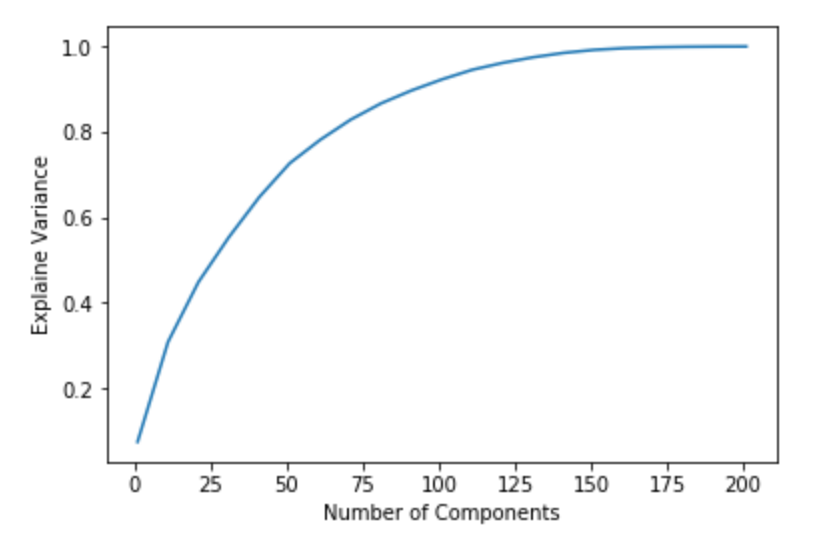
\includegraphics[width=.5\textwidth]{pca_explain.png}
        \caption{Number of principal components and the explained variance}
        \label{fig:pca_explain}
\end{figure}

I experimentally determined if it was worth proceeding with PCA.  Using the
XGBoost gradient boosting module I defined a set of consistent hyper parameters,
which are shown in Table~\ref{tab:xgb_params}for comparison.  I trained the
model using the training data, 80\% of the full training dataset, and varied the
amount of components used during training. Predictions were made on the
validation set, 20\% of the original training dataset, and the AUROC were
calculated.  Figure~\ref{fig:pca_auc} shows how varying the number of principal
components affects the AUROC score. 

\begin{table}[h!]
\centering
\caption{XGBoost parameters}
\resizebox{.3\textwidth}{!}{
\begin{tabular}{|c|c|}
\hline
Parameter & Value \\ \hline\hline
n\_estimators & 1000 \\ \hline
tree\_method & gpu\_hist \\ \hline
predictor & gpu\_predictor \\ \hline
max\_depth & 3 \\ \hline
eval\_metric & auc \\ \hline
\end{tabular}
}
\label{tab:xgb_params}
\end{table}

\begin{figure}[h!]
    \centering
        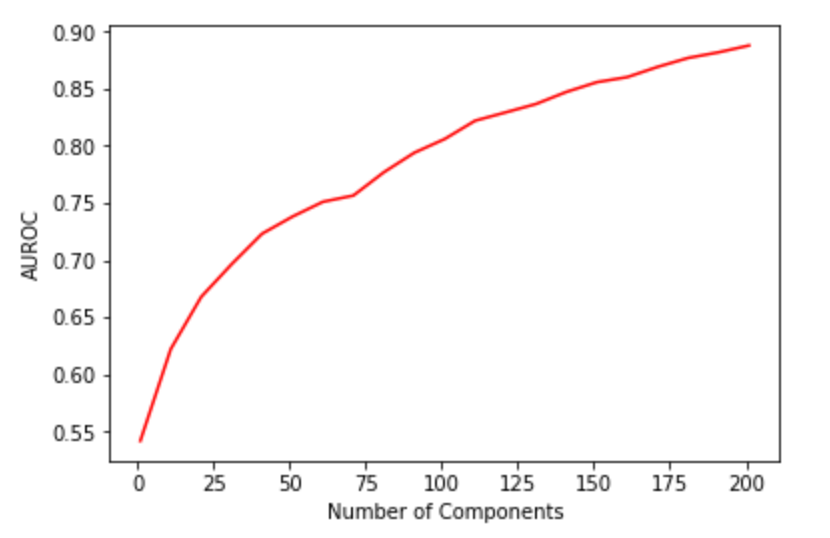
\includegraphics[width=.5\textwidth]{pca_auc.png}
        \caption{AUROC scores have a positive correlation to the number of
principal components}
        \label{fig:pca_auc}
\end{figure}

The results in Figure~\ref{fig:pca_auc} led me away from PCA.  Using all the components
with XGBoost resulted in a fairly good AUROC at 0.887.  I decided to stick with the
XGBoost classifier and proceed with feature engineering.  As mentioned in the
previous section, I constructed two extra features.  Frequency distributions for
each of the features are plotted in Figure~\ref{fig:count_dist} and are colored by
class.

\begin{figure}[h!]
    \centering
    \begin{subfigure}[]{.4\textwidth}
        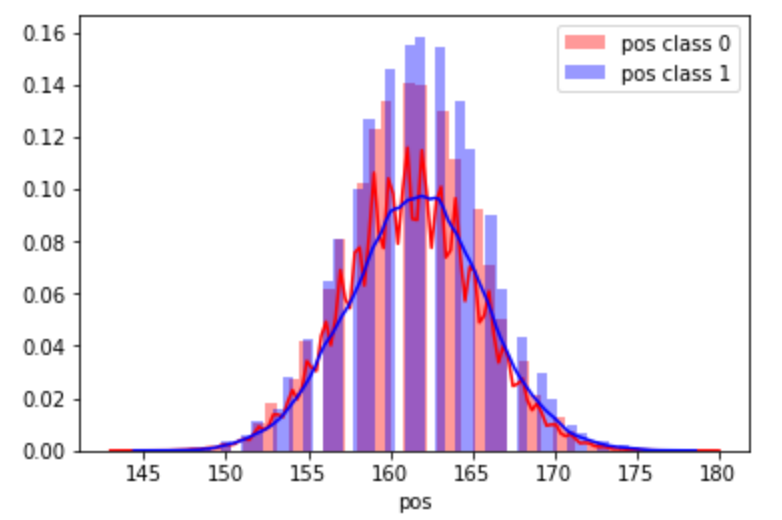
\includegraphics[width=\textwidth]{pos_dist.png}
        \caption{Distribution of positive numbers by class}
        \label{fig:pos_dist}
    \end{subfigure}
    \begin{subfigure}[]{.4\textwidth}
        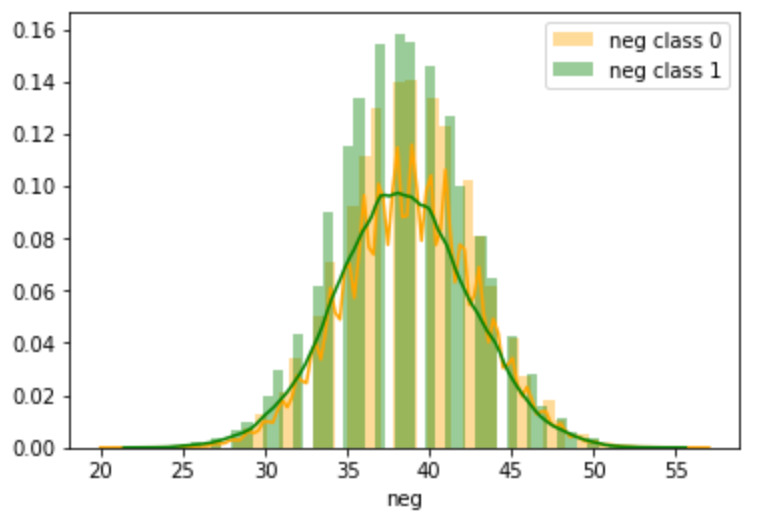
\includegraphics[width=\textwidth]{neg_dist.png}
        \caption{Distribution of negative numbers by class}
        \label{fig:neg_dist}
    \end{subfigure}
    \caption{Frequency distributions for positive and negative values colored by
class}
    \label{fig:count_dist}
\end{figure}

Figure~\ref{fig:count_dist} indicates that there are some differences
between class 0 and class 1 when looking at the total number of positive feature
values and the total number of negative feature values. The separation seen in
Figures~\ref{fig:pos_dist} and~\ref{fig:neg_dist} display more difference and
less overlap than any of the 200 original features.  As a result, I
hypothesized that adding these features to the model may help with training. 

Distributions of the longest positive and negative sequences with respect to
each class are shown in Figure~\ref{fig:count_dist}.  These two features were
constructed under the assumption that the features correspond to some type of
sequence data.  Again, I was trying to find features which show more separation
between the two classes than the original 200 features.

\begin{figure}[h!]
    \centering
    \begin{subfigure}[]{.4\textwidth}
        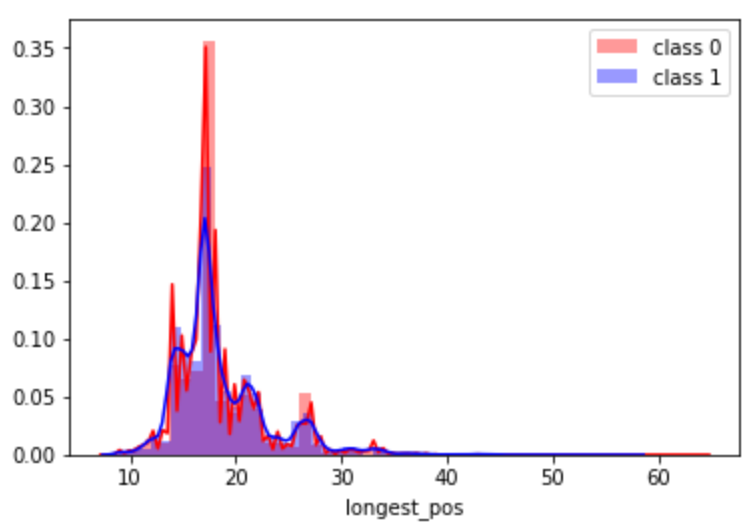
\includegraphics[width=\textwidth]{long_pos_dist.png}
        \caption{Distribution of positive numbers by class}
        \label{fig:pos_dist}
    \end{subfigure}
    \begin{subfigure}[]{.4\textwidth}
        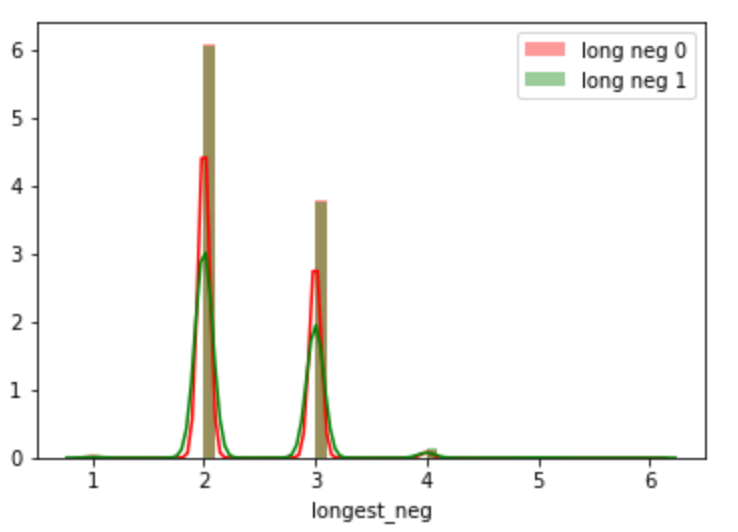
\includegraphics[width=\textwidth]{long_neg_dist.png}
        \caption{Distribution of negative numbers by class}
        \label{fig:neg_dist}
    \end{subfigure}
    \caption{Frequency distributions for longest positive sequence and longest
negative sequence values colored by class}
    \label{fig:count_dist}
\end{figure}

The resulting distributions for the longest positive and negative sequences are
different than the total count of positive and negative numbers as well as the
rest of the 200 features There are slight differences with respect to each class
which may help to improve the models.  Using this new feature may come with some
risk because it is likely that the feature order may have been randomized before
the datasets were released.  If that was the case, the longest positive and
negative sequences will be different and possibly irrelevant.

The hyper parameters for the XGBoost classifier were tuned using GridSearchCV
from sklearn.  GridSearchCV does not support GPU tree\_methods and so the search
was done on the CPU tree methods.  Final models were constructed using the GPU
versions of the hyper parameters for speed gains.  Finalize parameters are shown
in Table~\ref{tab:xgb_params}.  Some extra tuning of hyper parameters were done
to account for possible differences in the tree\_methods between the CPU and GPU
implementation.  The best hyper parameters were chosen based on AUROC scores
for the validation set.  It is likely that overfitting could have occurred and
that good performance on the validation set does not indicate a good ability for
the model to generalize to the test set.  In order to mitigate some overfitting
issues I used cross validation.  Overall, the AUROC scores from validation were
similar, out to four decimal places, to the resulting public score.  This made
me confident that any overfitting that may have occurred was not too extreme.

\begin{table}[h!]
\centering
\caption{XGBoost final hyper parameters}
\resizebox{.3\textwidth}{!}{
\begin{tabular}{|c|c|}
\hline
Parameter & Value \\ \hline\hline
n\_estimators & 3500 \\ \hline
tree\_method & gpu\_exact \\ \hline
predictor & gpu\_predictor \\ \hline
max\_depth & 2 \\ \hline
eval\_metric & auc \\ \hline
\end{tabular}
}
\label{tab:xgb_params}
\end{table}

When the hyper parameters were finalized, the XGBoost classifier was trained on
the full training dataset using the hyper parameters from
Table~\ref{tab:xgb_params}.  The classifier was then used to make predictions on
the test set.  The predictions were uploaded and the public score is shown below
in Table~\ref{tab:final}

\begin{table}[h!]
\centering
\caption{Final public results}
\resizebox{.4\textwidth}{!}{
\begin{tabular}{|c|c|}
\hline
Model & Best Public Score \\ \hline \hline
1D CNN & 0.833 \\ \hline
LSTM & 0.829 \\ \hline
PCA XGBoost & 0.882 \\ \hline
XGBoost w/ feat engineering & 0.899 \\ \hline
\end{tabular}
}
\label{tab:final}
\end{table}

In addition to XGBoost, PCA, and some feature engineering, I implemented a 1D CNN
and an LSTM as an exploratory experiment.  The initial submissions for both the
1D CNN and LSTM resulted in the scores seen in in Table~\ref{tab:final}.  In an
attempt to achieve higher scores for both models I ran then through more epochs.
While their performance on the validation sets increased considerably with more
epochs, I suspected overfitting to be an issue.  The performance on the public
leader board dropped and was lower than the previous models which were
constructed on less epochs.  These models were not pursued any further.  Feature
engineering along with the XGBoost classifier for which hyper parameters were
tuned gave me the best public score.

\section{Conclusion}

As of 3/14/2019 the top score on the leader board is 0.924.  My best score is
0.899 which was the result of the XGBoost classifier with some added features.
It is hard for me to have a confident idea of my models ability to win because
of the fact that still little is known about the data, the 200 features, and
what each class represents.%  Currently, there is a considerable amount of peopel with score ranging from 0.888 to 0.900

\end{document}
